% Vietnamese translation for OI Public Library
% Source-PDF: IOI中国国家候选队论文/2001/李源.pdf
\documentclass[11pt]{article}
\usepackage{oipl-vn}
\usepackage{tikz}
\usetikzlibrary{arrows.meta,fit,positioning}

\title{Liệt kê cây có hướng}
\author{Li Yuan}
\date{}

\newcommand{\Leaf}{\mathsf{L}}
\newcommand{\Tree}[1]{\mathsf{T}(#1)}
\newcommand{\Path}{\mathsf{P}}

\tikzset{
  treev/.style={circle,fill=black,inner sep=1.45pt},
  cutbox/.style={draw,dashed,rounded corners=1pt,inner sep=3pt},
  stepArrow/.style={-{Latex[length=2mm]},thick}
}

\newcommand{\TinyTreeA}{%
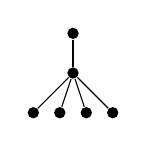
\begin{tikzpicture}[baseline=-0.5ex,scale=0.56]
  \node[treev] (r) at (0,1.8) {};
  \node[treev] (a) at (0,0.9) {};
  \foreach \x/\n in {-0.9/b,-0.3/c,0.3/d,0.9/e}
    \node[treev] (\n) at (\x,0) {};
  \draw (r)--(a);
  \foreach \n in {b,c,d,e} \draw (a)--(\n);
\end{tikzpicture}}

\newcommand{\TinyTreeB}{%
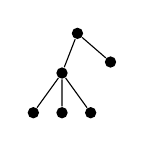
\begin{tikzpicture}[baseline=-0.5ex,scale=0.56]
  \node[treev] (r) at (0,1.8) {};
  \node[treev] (a) at (-0.35,0.9) {};
  \node[treev] (f) at (0.75,1.15) {};
  \foreach \x/\n in {-1.0/b,-0.35/c,0.3/d}
    \node[treev] (\n) at (\x,0) {};
  \draw (r)--(a) (r)--(f);
  \foreach \n in {b,c,d} \draw (a)--(\n);
\end{tikzpicture}}

\newcommand{\TinyTreeC}{%
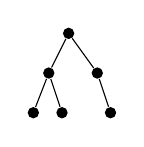
\begin{tikzpicture}[baseline=-0.5ex,scale=0.56]
  \node[treev] (r) at (0,1.8) {};
  \node[treev] (a) at (-0.45,0.9) {};
  \node[treev] (b) at (0.65,0.9) {};
  \node[treev] (c) at (-0.8,0) {};
  \node[treev] (d) at (-0.15,0) {};
  \node[treev] (e) at (0.95,0) {};
  \draw (r)--(a) (r)--(b) (a)--(c) (a)--(d) (b)--(e);
\end{tikzpicture}}

\begin{document}
\maketitle

\origtitle{Enumerating directed trees}
\sourcepath{IOI China candidate team papers / 2001 / Li Yuan.pdf}

\section{Dẫn nhập}

Cây là một cấu trúc phi tuyến rất quan trọng trong thuật toán máy tính. Ngay
cả khi tạm gác những ứng dụng rộng rãi của cây sang một bên, việc suy nghĩ và
nghiên cứu riêng hình dạng của cây cũng là một quá trình thú vị và có tính
thử thách.

Trong tài liệu này, ``cây có hướng'' được hiểu là cây có gốc; các cạnh có thể
xem như hướng từ gốc xuống con. Với bốn đỉnh, chẳng hạn, ta đã có các dạng
cơ bản sau nếu viết \(\Leaf\) là lá và \(\Tree{S_1,\ldots,S_k}\) là một gốc có
các cây con \(S_1,\ldots,S_k\):
\[
  \Tree{\Tree{\Tree{\Leaf}}},\qquad
  \Tree{\Tree{\Leaf,\Leaf}},\qquad
  \Tree{\Tree{\Leaf},\Leaf},\qquad
  \Tree{\Leaf,\Leaf,\Leaf}.
\]

\section{Thuật toán liệt kê}

Cách làm thông thường là tìm kiếm rồi khử trùng:
\[
  \text{sinh trạng thái}
  \longrightarrow
  \text{xét các trạng thái đẳng cấu}
  \longrightarrow
  \text{so với nghiệm đã có}
  \longrightarrow
  \text{thêm vào tập nghiệm}.
\]
Phần còn lại trình bày một thuật toán xây dựng có thể sinh tất cả cây có
hướng với số đỉnh và độ sâu cho trước mà không sinh lặp.

Hai ý chính của thuật toán là:
\begin{itemize}
  \item tính không lặp đến từ một định nghĩa thứ tự giữa các cây;
  \item tính không sót đến từ quy tắc biến đổi từ cây hiện tại sang cây kế
  tiếp trong thứ tự đó.
\end{itemize}

\section{Định nghĩa thứ tự của cây}

Ta đặt ra một quan hệ ``lớn hơn'' giữa các cây, nhờ đó các cấu trúc cây khác
nhau trở thành một dãy có thứ tự. Khi so sánh hai cây \(A\) và \(B\), mọi cây
con của chúng cũng được sắp từ lớn đến nhỏ theo chính quan hệ này.

Quy tắc so sánh là:
\begin{enumerate}
  \item Nếu độ sâu của \(A\) lớn hơn độ sâu của \(B\), thì \(A>B\). Nếu nhỏ
  hơn, thì \(A<B\).
  \item Nếu hai độ sâu bằng nhau, so sánh số đỉnh. Cây có nhiều đỉnh hơn là
  cây lớn hơn.
  \item Nếu cả độ sâu lẫn số đỉnh đều bằng nhau, so sánh lần lượt các cây con
  đã được sắp theo thứ tự giảm dần. Tại vị trí đầu tiên mà hai cây con khác
  nhau, cây chứa cây con lớn hơn là cây lớn hơn. Nếu cặp cây con hiện tại
  bằng nhau thì xét cặp kế tiếp.
\end{enumerate}

Như vậy, với mọi \(d\) và \(n\), toàn bộ cây có hướng có độ sâu \(d\) và số
đỉnh \(n\) có thể được xếp từ lớn đến nhỏ thành một dãy. Ví dụ với
\(d=3,n=6\), dãy là:
\[
\begin{array}{ccl}
1 &:& \Tree{\Tree{\Leaf,\Leaf,\Leaf,\Leaf}},\\
2 &:& \Tree{\Tree{\Leaf,\Leaf,\Leaf},\Leaf},\\
3 &:& \Tree{\Tree{\Leaf,\Leaf},\Tree{\Leaf}},\\
4 &:& \Tree{\Tree{\Leaf,\Leaf},\Leaf,\Leaf},\\
5 &:& \Tree{\Tree{\Leaf},\Tree{\Leaf},\Leaf},\\
6 &:& \Tree{\Tree{\Leaf},\Leaf,\Leaf,\Leaf}.
\end{array}
\]
Ba dạng đầu của dãy trên có thể hình dung như sau:
\[
  \TinyTreeA\quad \longrightarrow \quad
  \TinyTreeB\quad \longrightarrow \quad
  \TinyTreeC .
\]

Với \(d,n\) bất kỳ, cây đầu và cây cuối của dãy cũng dễ xác định:
\begin{itemize}
  \item Cây lớn nhất là một đường đi gồm \(d-1\) đỉnh tính từ gốc đến đỉnh
  ngay trên tầng cuối; đỉnh này có \(n-d+1\) lá.
  \item Cây nhỏ nhất là một đường đi đạt độ sâu \(d\), còn \(n-d\) đỉnh còn
  lại đều là lá trực tiếp của gốc.
\end{itemize}

Bài toán vì thế chuyển thành câu hỏi: theo định nghĩa thứ tự trên, có thể tìm
một quy tắc biến đổi để bắt đầu từ cây lớn nhất và liên tục sinh cây kế tiếp,
không sót và không lặp, cho đến cây nhỏ nhất hay không?

\section{Quá trình biến đổi}

Chuyển từ một cây trong dãy sang cây kế tiếp là một quá trình làm cây nhỏ đi.
Trong quá trình đó, ít nhất một cây con bị làm nhỏ đi. Việc làm nhỏ được thực
hiện bằng cách lấy đi một đỉnh con của nó; trong các hình gốc, cây con bị làm
nhỏ được đánh dấu bằng khung nét đứt.

Sau khi đỉnh bị lấy đi, một số cây con đứng sau cây con vừa bị làm nhỏ sẽ nhận
đỉnh này hoặc được tổ hợp lại. Chúng có thể lớn lên một cách thích hợp. Tuy
nhiên, vì trong phép so sánh kích thước cây, vị trí của chúng thấp hơn vị trí
của cây con vừa bị làm nhỏ, nên xét toàn cục, cả cây vẫn nhỏ đi.

Quá trình biến đổi được chia thành hai phần:
\begin{itemize}
  \item Quy trình I: tìm đỉnh sẽ bị xóa.
  \item Quy trình II: ghép lại đỉnh bị xóa vào các cây con đứng sau.
\end{itemize}

\section{Quy trình I: tìm đỉnh bị xóa}

Khi chọn đỉnh bị xóa, ảnh hưởng của việc làm nhỏ cây con chứa nó đối với toàn
bộ cây phải nhỏ nhất có thể. Nhờ vậy, sau biến đổi ta thu được đúng cây kề
tiếp trong dãy, chứ không nhảy qua nhiều cây.

Từ yêu cầu đó có hai nhận xét trực tiếp:
\begin{itemize}
  \item Đỉnh bị lấy đi chắc chắn là một lá.
  \item Với nhiều cây con ngang hàng, phải tìm từ phải sang trái.
\end{itemize}

\subsection{Thuật toán của quy trình I}

Bắt đầu từ gốc. Trong các con của đỉnh hiện tại, tìm từ phải sang trái con đầu
tiên không phải là lá, rồi đi tiếp xuống con đó. Lặp lại cho đến khi gặp một
đỉnh mà mọi con của nó đều là lá. Khi đó ứng viên tự nhiên là con cuối cùng
của đỉnh này.

Tuy nhiên, chưa thể luôn xem con cuối cùng ấy là đỉnh cần xóa. Giả sử ứng
viên \(A\) là con duy nhất của cha \(B\). Nếu xóa \(A\) khỏi \(B\), độ sâu
của cây con gốc \(B\) giảm đi \(1\). Vì trong định nghĩa thứ tự, độ sâu được
ưu tiên hơn số đỉnh, ta nên ưu tiên xóa một đỉnh sao cho độ sâu của cây con
bị tác động không đổi.

Do đó, sau khi tìm được \(A\), phải truy ngược theo các cha cho đến khi độ
sâu của cây con dưới đỉnh hiện tại không đổi khi xóa \(A\). Trong lúc truy
ngược, nếu đi qua một đỉnh vẫn còn một con khác, thì bỏ ứng viên cũ và chọn
con còn lại đó làm đỉnh bị xóa. Trong hình minh họa của tài liệu gốc, khi đi
ngược từ \(A\) qua \(B\) đến \(C\), vì \(C\) còn một con \(E\), thuật toán
đổi mục tiêu từ \(A\) sang \(E\).

\[
\begin{tikzpicture}[scale=0.72]
  \node[treev,label=above:{\(\)}] (r) at (0,4) {};
  \node[treev,label=right:{\(D\)}] (D) at (0,3.25) {};
  \node[treev] (l1) at (-1.0,2.4) {};
  \node[treev,label=left:{\(C\)}] (C) at (0.15,2.4) {};
  \node[treev] (l2) at (-1.35,1.55) {};
  \node[treev,label=left:{\(B\)}] (B) at (0.25,1.55) {};
  \node[treev] (l3) at (-1.7,0.7) {};
  \node[treev,label=right:{\(A\)}] (A) at (0.45,0.7) {};
  \node[treev,label=right:{\(E\)}] (E) at (1.35,2.05) {};
  \draw (r)--(D) (D)--(l1) (D)--(C) (l1)--(l2) (l2)--(l3)
        (C)--(B) (B)--(A) (C)--(E);
  \node[cutbox,fit=(B) (A)] {};
  \draw[stepArrow,blue] (0.9,0.85) .. controls (1.25,1.25) and (1.15,1.9) .. (0.55,2.25);
  \draw[stepArrow,blue] (0.75,2.55) -- (1.15,2.15);
  \node[align=left] at (4.2,2.5)
    {Nếu xóa \(A\), độ sâu dưới \(B\) và \(C\) đều đổi.\\
     Khi truy ngược đến \(C\), chọn \(E\) làm mục tiêu.};
\end{tikzpicture}
\]

\section{Quy trình II: ghép lại đỉnh bị xóa}

Sau khi tìm và xóa đỉnh mục tiêu, cần xử lý tiếp để tạo thành một cây mới.
Nguyên tắc quan trọng là: làm cả cây nhỏ đi, nhưng mức giảm phải là nhỏ nhất.

Sau khi xóa một đỉnh có hai khả năng:
\begin{itemize}
  \item độ sâu của cây con hiện tại không đổi, còn số đỉnh giảm;
  \item độ sâu của cây con hiện tại giảm.
\end{itemize}

\subsection{Độ sâu cây con không đổi}

Trong trường hợp này, xét các cây con đứng sau cây con vừa bị sửa. Ta tổ hợp
lại chúng, đồng thời đưa đỉnh vừa xóa vào, sao cho mọi cây con ở phần sau
không lớn hơn cây con hiện tại và bản thân phần sau là lớn nhất có thể.

\[
\begin{tikzpicture}[scale=0.72]
  \node[treev] (r1) at (0,2.8) {};
  \node[treev] (a1) at (-0.9,1.75) {};
  \node[treev] (x1) at (-1.35,0.85) {};
  \node[treev] (y1) at (-0.55,0.85) {};
  \node[treev] (b1) at (0,1.75) {};
  \node[treev] (c1) at (0.75,1.75) {};
  \node[treev] (d1) at (1.45,1.75) {};
  \draw (r1)--(a1) (a1)--(x1) (a1)--(y1) (r1)--(b1) (r1)--(c1) (r1)--(d1);
  \node[cutbox,fit=(y1)] {};
  \node[below=0.2cm of x1,align=center] {xóa lá,\\cây con nhỏ đi};

  \draw[stepArrow] (2.0,1.75) -- (3.0,1.75);

  \node[treev] (r2) at (4.0,2.8) {};
  \node[treev] (a2) at (3.2,1.75) {};
  \node[treev] (x2) at (2.8,0.85) {};
  \node[treev] (b2) at (4.0,1.75) {};
  \node[treev] (c2) at (4.65,1.75) {};
  \node[treev] (d2) at (5.3,1.75) {};
  \node[treev] (extra) at (5.95,1.75) {};
  \draw (r2)--(a2) (a2)--(x2) (r2)--(b2) (r2)--(c2) (r2)--(d2);
  \node[cutbox,fit=(b2) (c2) (d2)] {};
  \node at (5.65,1.75) {\(+\)};
  \node[below=0.2cm of x2,align=center] {tổ hợp lại phần sau\\để đạt lớn nhất};

  \draw[stepArrow] (6.35,1.75) -- (7.35,1.75);

  \node[treev] (r3) at (8.7,2.8) {};
  \node[treev] (a3) at (7.9,1.75) {};
  \node[treev] (x3) at (7.5,0.85) {};
  \node[treev] (b3) at (8.7,1.75) {};
  \node[treev] (bb3) at (8.7,0.85) {};
  \node[treev] (c3) at (9.55,1.75) {};
  \node[treev] (cc3) at (9.95,0.85) {};
  \draw (r3)--(a3) (a3)--(x3) (r3)--(b3) (b3)--(bb3) (r3)--(c3) (c3)--(cc3);
  \node[below=0.2cm of bb3,align=center] {biến đổi xong};
\end{tikzpicture}
\]

\subsection{Độ sâu cây con giảm}

Nếu xóa đỉnh làm độ sâu của cây con thay đổi, ta phải xử lý theo chuỗi từ
dưới lên. Xét ví dụ trong tài liệu: \(F\) là đỉnh cần xóa khỏi cha; các cây
con gốc \(C\) và \(E\) sẽ bị giảm độ sâu nên cần xử lý tiếp.

Trước hết xóa \(F\), rồi xử lý \(E\) cùng các anh em của nó; ở ví dụ này phần
ấy rỗng. Ghép phần này với \(F\) và tổ hợp lại dưới gốc \(C\). Tiếp đó xử lý
\(C\) cùng anh em của nó, chẳng hạn \(D\), và toàn bộ các cây con dưới \(C\);
tổ hợp lại dưới cha \(B\). Sau bước này thu được cây mới.

\[
\begin{tikzpicture}[scale=0.72]
  \node[treev,label=above:{\(A\)}] (A1) at (0,4) {};
  \node[treev,label=left:{\(B\)}] (B1) at (0,3.25) {};
  \node[treev] (L1) at (-0.75,2.35) {};
  \node[treev,label=right:{\(C\)}] (C1) at (0.5,2.35) {};
  \node[treev,label=right:{\(D\)}] (D1) at (1.35,2.9) {};
  \node[treev] (LL1) at (-1.05,1.45) {};
  \node[treev,label=left:{\(E\)}] (E1) at (0.25,1.45) {};
  \node[treev,label=right:{\(F\)}] (F1) at (0.75,0.65) {};
  \draw (A1)--(B1) (B1)--(L1) (B1)--(C1) (B1)--(D1)
        (L1)--(LL1) (C1)--(E1) (C1)--(F1);
  \node[below=0.1cm of LL1,align=center] {xóa \(F\);\\\(C,E\) cần xử lý};

  \draw[stepArrow] (1.8,2.2) -- (2.8,2.2);

  \node[treev,label=above:{\(A\)}] (A2) at (4.0,4) {};
  \node[treev,label=left:{\(B\)}] (B2) at (4.0,3.25) {};
  \node[treev] (L2) at (3.25,2.35) {};
  \node[treev,label=right:{\(C\)}] (C2) at (4.5,2.35) {};
  \node[treev,label=right:{\(D\)}] (D2) at (5.35,2.9) {};
  \node[treev] (LL2) at (2.95,1.45) {};
  \node[treev,label=left:{\(E\)}] (E2) at (4.15,1.45) {};
  \node[treev,label=right:{\(F\)}] (F2) at (4.9,1.45) {};
  \draw (A2)--(B2) (B2)--(L2) (B2)--(C2) (B2)--(D2)
        (L2)--(LL2) (C2)--(E2) (C2)--(F2);
  \node[below=0.1cm of LL2,align=center] {ghép \(F\) lại\\dưới \(C\)};

  \draw[stepArrow] (5.8,2.2) -- (6.8,2.2);

  \node[treev,label=above:{\(A\)}] (A3) at (8.2,4) {};
  \node[treev,label=left:{\(B\)}] (B3) at (8.2,3.25) {};
  \node[treev] (L3) at (7.45,2.35) {};
  \node[treev,label=right:{\(C\)}] (C3) at (8.65,2.35) {};
  \node[treev] (LL3) at (7.15,1.45) {};
  \node[treev,label=left:{\(E\)}] (E3) at (8.15,1.45) {};
  \node[treev,label=below:{\(F\)}] (F3) at (8.65,1.45) {};
  \node[treev,label=right:{\(D\)}] (D3) at (9.15,1.45) {};
  \draw (A3)--(B3) (B3)--(L3) (L3)--(LL3) (B3)--(C3)
        (C3)--(E3) (C3)--(F3) (C3)--(D3);
  \node[below=0.1cm of LL3,align=center] {xử lý \(C\) và \(D\);\\thu được cây mới};
\end{tikzpicture}
\]

\section{Thuật toán tổng quát}

Thuật toán liệt kê cây có gốc có thể viết ở mức cao như sau:
\[
\begin{array}{ll}
1. & \text{Đọc } d,n.\\
2. & \text{Tìm cây đầu tiên, tức cây lớn nhất.}\\
3. & \text{Trong khi chưa sinh hết các cây:}\\
4. & \quad \text{tìm đỉnh cần xóa } target;\\
5. & \quad \text{xóa } target;\\
6. & \quad \text{biến đổi cây theo một trong hai trường hợp của Quy trình II.}
\end{array}
\]
Điều kiện dừng có thể lấy từ tổng số cây do một thuật toán đếm cung cấp, hoặc
có thể xác định trước cây nhỏ nhất rồi dừng khi đạt đến cây đó.

\section{Kết luận và độ phức tạp}

Mặc dù quá trình biến đổi ở trên trông khá phức tạp, bản chất của nó dựa trên
một quy luật gọn và chặt chẽ. Khi nghiên cứu kỹ, có thể thấy nó hài hòa với
thứ tự đã định nghĩa, khá giống phép giảm số tự nhiên có mượn.

Chẳng hạn, để biến \(2000\) thành số tự nhiên nhỏ hơn nó nhưng chênh lệch ít
nhất, ta có thể nhìn quá trình như sau:
\[
  2000 \longrightarrow 1000 \longrightarrow 1999.
\]
Bước đầu tiên làm giảm chữ số quan trọng hơn; bước thứ hai đưa phần phía sau
lên lớn nhất có thể. Với cây có hướng cũng vậy: ta tìm một lá từ phải sang
trái để xóa, rồi biến đổi các cây con còn lại, tương tự việc đổi các chữ số
\(0\) phía sau thành \(9\), để mức giảm của toàn cây là nhỏ nhất. Kết quả là
cây kế tiếp trong dãy.

Thuật toán trên sinh được, với độ sâu \(d\) và số đỉnh \(n\) cho trước, mọi
hình dạng cây có hướng theo thứ tự từ lớn đến nhỏ. Các thao tác sao chép cây
và duyệt cây đều có độ phức tạp \(O(n)\). Vì trong quá trình sinh hoàn toàn
không có lặp, thời gian chạy chủ yếu phụ thuộc vào tổng số hình dạng cây khác
nhau.

Ứng dụng trực tiếp nhất của thuật toán là bài toán cây không gốc. Bảng sau là
một tham khảo trực quan về thời gian, so sánh chương trình sinh theo thuật
toán xây dựng với phương pháp tìm kiếm. Môi trường thử nghiệm trong tài liệu
gốc là PIII 500MHz, 192MB RAM, Borland Pascal 7.0; đơn vị thời gian là giây.

\begin{center}
\scriptsize
\(\begin{array}{c|rrrrrrrrrr}
N & 11 & 12 & 13 & 14 & 15 & 16 & 17 & 18 & 19 & 20\\ \hline
\text{Xây dựng} & 0.05 & 0.05 & 0.11 & 0.16 & 0.49 & 1.21 & 3.19 & 8.52 & 23.08 & 62.91\\
\text{Tìm kiếm} & 0.27 & 0.71 & 2.09 & 6.04 & 17.69 & 51.92 & 152.20 & {-} & {-} & {-}
\end{array}\)
\end{center}

\end{document}
